\documentclass{file/TA-ITS}
%Ridho Nur Rohman Wijaya

\makeatletter
\def\cleardoublepage{\clearpage%
	\if@twoside
	\ifodd\c@page\else
	\vspace*{\fill}
	\hfill
	\begin{center}
		\emph{ }
	\end{center}
	\vspace{\fill}
	\thispagestyle{empty}
	\newpage
	\if@twocolumn\hbox{}\newpage\fi
	\fi
	\fi
}
\makeatother
\newtheorem{definisi}{Definisi}[section]
\newtheorem{teorema}[definisi]{Teorema}
\newtheorem{thm}{Teorema}[section]
\newtheorem{lemma}[definisi]{Lemma}
\newtheorem{lemmas}[thm]{Lemma}
\newtheorem{cor}[definisi]{Akibat}
\theoremstyle{definition}
\newtheorem{con}[definisi]{Contoh}
\theoremstyle{definition}
\theoremstyle{plain}
\newtheorem{prop}[definisi]{Proposisi}
\renewcommand{\proofname}{Bukti}
\renewcommand{\thethm}{\arabic{chapter}.\arabic{thm}}

\newcommand{\norm}[1]{\left\|#1\right\|} % Fungsi norm (||x||)

\newcommand\firstPar{0.75cm} % Indentasi 0.75cm pada tiap paragraf (manual untuk hspace)
\setlength{\parindent}{0.75cm} % Indentasi 0.75cm pada tiap paragraf

\usepackage{fancyhdr}
\pagestyle{fancy}
\renewcommand{\headrulewidth}{0pt}
\fancyhf{}
\usepackage{ifthen}
\fancyfoot[R]{\thepage}

\usepackage[labelsep=quad]{caption}
\captionsetup[table]{skip=5pt}

\usepackage{multirow}
\usepackage{longtable}
\usepackage{tikz}
%%% Pewarnaan code
\usepackage{color}
\usepackage{listings}

\definecolor{codegreen}{rgb}{0,0.6,0}
\definecolor{codeblack}{rgb}{0,0,0}
\definecolor{codepurple}{rgb}{0.58,0,0.82}
\definecolor{backcolour}{rgb}{0.95,0.95,0.92}

\lstdefinestyle{mystyle}{
    commentstyle=\color{codegreen},
    keywordstyle=\color{magenta},
    numberstyle=\tiny\color{codeblack},
    stringstyle=\color{codepurple},
    basicstyle=\ttfamily\footnotesize,
    breakatwhitespace=false,         
    breaklines=true,                 
    captionpos=b,                    
    keepspaces=true,                 
    numbers=left,                    
    numbersep=5pt,                  
    showspaces=false,                
    showstringspaces=false,
    showtabs=false,                  
    tabsize=2
}
%%% Pewarnaan code

\hypersetup{ % Merubah warna link
    colorlinks,
    linkcolor={black},
    citecolor={black},
    urlcolor={black}
}

% \tolerance=1
% \emergencystretch = \maxdimen
% \hyphenpenalty=10000
% \hbadness=1000

\newcommand{\Real}{\mathbb{R}}
\newcommand{\N}{\mathbb{N}}
\newcommand{\Z}{\mathbb{Z}}
\newcommand{\Q}{\mathbb{Q}}
\newcommand{\defeq}{\overset{\mathrm{def}}{=}}

\begin{document}

% input data
\Judul{Optimisasi Jadwal Jaringan Bus di Terminal Purabaya Menggunakan Aljabar Max-Plus}

\JudulEng{Optimization of Bus Network Scheduling at Purabaya Terminal Using Max-Plus Algebra}

\Nama{Teosofi Hidayah Agung}

\NamaKecil{Teosofi Hidayah Agung}

\NRP{5002221132}

\Departemen{Matematika}

\Department{Mathematics}

\BidangStudi{Aljabar dan Analisis}

\Bulan{November} % Masuk lembar pengesahan

\Tahun{2024}

\TanggalDisetujui{22 November 2024} % Masuk lembar orisinilitas

\Fakultas{Sains dan Analitika Data}

\SingkatanFakultas{FSAD}

\Faculty{Scientics}

\SingkatanFakultasEng{SCIENTICS}

\Pembimbing{Pembimbing 1}
          {} % Isi {} untuk pembimbing 2
		   

\NIPPembimbing{NIP}
{} % Isi {} untuk pembimbing 2
              
              
\Penguji{Penguji 1}
        {Penguji 2}
        {Penguji 3}

\NIPPenguji{NIP Penguji 1}
           {NIP Penguji 2}
           {NIP Penguji 3}
\Kadep{Nama Kadept}

\NIPKadep{NIP Pak Kadept}
\BagianAwal
\LembarJudul
\LembarPengesahan
%%%%%%%%%%%%%%%%%%%%%%%%  Abstrak  %%%%%%%%%%%%%%%5%%%%%%%%%%

\begin{Abstrak}
Transportasi publik merupakan salah satu komponen penting dalam mendukung mobilitas masyarakat perkotaan. Terminal Purabaya memiliki peran strategis dalam sistem transportasi di Surabaya, namun pengelolaan jadwal bus yang kurang optimal dapat menyebabkan ketidakefisienan waktu tunggu penumpang dan pengoperasian bus. Penelitian ini bertujuan mengoptimalkan jadwal jaringan bus di Terminal Purabaya menggunakan pendekatan aljabar max-plus. Pendekatan ini memodelkan jadwal sebagai sistem linier max-plus yang mempertimbangkan waktu siklus (\textit{cyclicity}) dan waktu transient untuk memastikan efisiensi. Hasil simulasi diharapkan dapat meningkatkan akurasi dan efisiensi operasional bus.

\katakunci{Optimasi jadwal, aljabar max-plus, jaringan bus, efisiensi transportasi.}
\end{Abstrak}

\begin{Abstract}
Public transportation is a critical component supporting urban mobility. Purabaya Terminal plays a strategic role in Surabaya's transport system; however, suboptimal bus schedule management leads to inefficiencies in passenger waiting times and bus operations. This study aims to optimize the bus network schedule at Purabaya Terminal using the max-plus algebra approach. This approach models the schedule as a max-plus linear system, considering cyclicity and transient times to ensure efficiency. The simulation results are expected to enhance the accuracy and operational efficiency of bus services.

\keywords{Schedule optimization, max-plus algebra, bus network, transport efficiency.}
\end{Abstract}

%%%%%%%%%%%%%%%%%%%%%%%%  Abstrak  %%%%%%%%%%%%%%%5%%%%%%%%%%

%%%%%%%%%%%%%%%%%%%%%%%%  Daftar  %%%%%%%%%%%%%%%5%%%%%%%%%%

\DaftarIsi\raggedbottom

\DaftarGambar

\DaftarTabel

\DaftarSimbol
\begin{flushleft}
\begin{tabular}{lrl}

$\oplus$ &:& Operasi \textit{max} dalam aljabar max-plus \\

$\otimes$ &:& Operasi \textit{plus} dalam aljabar max-plus \\

$\varepsilon$ &:& Elemen netral untuk operasi $\oplus$, yaitu $-\infty$ \\

$e$ &:& Elemen satuan untuk operasi $\otimes$, yaitu $0$ \\

$\mathbf{A} \otimes \mathbf{x}$ &:& Hasil kali matriks $\mathbf{A}$ dengan vektor $\mathbf{x}$ pada aljabar max-plus \\

$\lambda$ &:& Nilai eigen dalam aljabar max-plus \\

$\mathbb{R}_{\max}$ &:& Himpunan bilangan real diperluas dengan $-\infty$ dalam aljabar max-plus \\

$\mathbb{R}_{\max}^n$ &:& Ruang vektor berdimensi $n$ dalam aljabar max-plus \\

$[\mathbf{A}^k]_{ij}$ &:& Elemen $(i,j)$ dari matriks $\mathbf{A}$ pangkat $k$ \\

\end{tabular}
\end{flushleft}
%%%%%%%%%%%%%%%%%%%%%%%%  Daftar  %%%%%%%%%%%%%%%5%%%%%%%%%%

\BagianInti

%%%%%%%%%%%%%%%%%%%%%%%%  Bab I  %%%%%%%%%%%%%%%5%%%%%%%%%%
\chapter{PENDAHULUAN}
\section{Latar Belakang}
\indent Transportasi umum merupakan salah satu kebutuhan utama masyarakat perkotaan untuk mendukung mobilitas sehari-hari. Di kota besar seperti Surabaya, keberadaan transportasi umum yang efisien dan terjadwal dengan baik sangat penting untuk mengurangi kemacetan, menghemat waktu perjalanan, serta meningkatkan kualitas hidup masyarakat. Salah satu transportasi umum yang menjadi andalan di Surabaya adalah Suroboyo Bus, yang dikenal dengan inovasi ramah lingkungannya dan upaya meningkatkan minat masyarakat menggunakan transportasi umum.

Transportasi ini diresmikan pada 7 April 2018 di Gedung Siola, dimana memiliki kapasitas 67 penumpang dan beroperasi setiap hari mulai pukul 06.00 hingga 22.00 WIB. Salah satu keunikan dari layanan ini adalah sistem pembayarannya, yang memanfaatkan sampah plastik. Ide ini muncul sebagai solusi untuk mengatasi permasalahan sampah plastik di Surabaya, yang setiap tahunnya terus meningkat. Kota Pahlawan sendiri menghasilkan sekitar 400 ton sampah plastik setiap harinya, sehingga langkah ini menjadi inovasi yang signifikan. Sampah plastik yang digunakan sebagai pembayaran akan dikumpulkan dan diserahkan ke Bank Sampah. Setelah itu, sampah tersebut dijual dan didaur ulang menjadi produk yang lebih bermanfaat. Suroboyo Bus menjadi satu-satunya transportasi umum di Indonesia yang menerapkan metode pembayaran unik ini. Sejak awal pengoperasiannya, masyarakat memberikan respons yang sangat positif. Mereka merasa antusias, nyaman, dan aman saat menggunakan layanan bus ini, menjadikannya salah satu inovasi transportasi yang layak diapresiasi.\cite{kusuma2020suroboyobusUU}

Menurut penelitian yang dilakukan \citeauthor{primadhanny2023pengaruhsuroboyobus} mengenai pengaruh pelayanan Suroboyo Bus terhadap kepuasan masyarakat Surabaya, hasilnya menunjukkan bahwa mayoritas responden merasa puas dengan pelayanan Suroboyo Bus. Hal ini menunjukkan bahwa layanan transportasi umum ini telah memberikan dampak positif bagi masyarakat Surabaya.

Tantangan dalam pengelolaan transportasi umum seperti Suroboyo Bus adalah memastikan jadwal keberangkatan dan kedatangan bus tetap terkoordinasi dengan baik. Ketidaktepatan jadwal dapat menyebabkan ketidakpuasan pengguna, berkurangnya efektivitas layanan, dan potensi penurunan jumlah pengguna. Oleh karena itu, diperlukan metode yang tepat untuk membuat model penjadwalan yang efisien dan dapat diandalkan.

Aljabar Max-Plus adalah salah satu metode matematika yang memiliki kemampuan untuk memodelkan sistem dinamis terdistribusi seperti jaringan transportasi. Metode ini memungkinkan analisis dan optimasi jadwal berdasarkan waktu operasional dan interval kedatangan sehingga dapat meminimalkan potensi keterlambatan dan meningkatkan efisiensi.

Melalui penelitian ini, diusulkan model penjadwalan Suroboyo Bus menggunakan Aljabar Max-Plus untuk memberikan solusi terukur dan efektif dalam menghadapi tantangan penjadwalan transportasi umum di kota Surabaya. Implementasi model ini diharapkan dapat mendukung keberlanjutan operasional Suroboyo Bus sekaligus memberikan dampak positif bagi penggunanya.

\section{Rumusan Masalah}
Berdasarkan latar belakang di atas, rumusan masalah yang akan dibahas dalam penelitian ini adalah sebagai berikut:

\begin{enumerate}
    \item Bagaimana memodelkan rute lalu lintas Suroboyo Bus menggunakan graf berarah dan berbobot?
    \item Bagaimana penerapan aljabar max-plus dalam perencanaan jadwal kedatangan dan keberangkatan Suroboyo Bus?
\end{enumerate}

\section{Batasan Masalah}
Untuk menjaga fokus penelitian dan memperjelas lingkup penelitian ini, terdapat beberapa batasan masalah yang ditetapkan, antara lain:

\begin{enumerate}
    \item Penelitian ini hanya akan memodelkan rute lalu lintas Suroboyo Bus dengan menggunakan pendekatan aljabar max-plus.
    \item Hanya jadwal kedatangan dan keberangkatan bus yang akan dianalisis, tanpa mempertimbangkan faktor eksternal seperti cuaca, kondisi jalan, atau perubahan kebijakan transportasi.
    \item Rute yang akan dianalisis adalah rute yang jalurnya masih berada dilingkungan kampus ITS, yakni Koridor R2, Koridor R4, dan Koridor SBT.
\end{enumerate}

\section{Tujuan}
Tujuan dari penelitian ini adalah untuk memberikan solusi yang lebih efisien dalam pengelolaan rute Suroboyo Bus dengan menggunakan metode aljabar max-plus. Secara khusus, penelitian ini bertujuan untuk:

\begin{enumerate}
    \item Memodelkan rute lalu lintas Suroboyo Bus menggunakan graf berarah dan berbobot.
    \item Mengoptimalkan jadwal operasional bus di terminal untuk meminimalkan waktu tunggu penumpang.
\end{enumerate}

\section{Manfaat}
Penelitian ini diharapkan memberikan beberapa manfaat, baik secara teoritis maupun praktis, di antaranya:

\begin{itemize}
    \item \textbf{Manfaat Teoritis}: Memberikan kontribusi pada pengembangan ilmu pengetahuan, khususnya dalam bidang transportasi dan matematika terapan melalui penerapan aljabar max-plus dalam perencanaan jadwal transportasi umum.
    \item \textbf{Manfaat Praktis}: Menjadikan pertimbangan Pemerintah kota Surabaya terhadap Suroboyo Bus mengoptimalkan jadwal keberangkatan dan kedatangan bus sehingga dapat meningkatkan efisiensi operasional.
\end{itemize}

\pagebreak
\chapter{TINJAUAN PUSTAKA}

\section{Terminologi Aljabar Max-Plus}
\indent Aljabar max-plus adalah perluasan dari aljabar biasa yang menggantikan operasi penjumlahan dan perkalian dengan operasi maksimum dan penjumlahan, Sebagaimana definisi yang diberikan sebagai berikut:
\begin{definisi}
    Diberikan himpunan $\Real_{\varepsilon} = \Real \cup \{\varepsilon\}$ dengan $\Real$ adalah himpunan bilangan real dan $\varepsilon\defeq-\infty$. Pada $\Real_{\varepsilon}$, didefinisikan dua operasi biner sebagai berikut:
    \begin{flalign}
        a \oplus b &\defeq \max\{a, b\} , \quad \forall a, b \in \Real_{\varepsilon} \label{eq:oplus} \\
        a \otimes b &\defeq a + b , \quad \forall a, b \in \Real_{\varepsilon} \label{eq:otimes}
    \end{flalign}
\end{definisi}
\noindent\cite{baccelli}

Selanjutnya akan ditunjukkan bahwa $\left(\Real_\varepsilon,\oplus,\otimes\right)$ adalah semiring dengan elemen netral $\varepsilon=-\infty$ dan elemen satuan $e=0$. Untuk setiap $a,b,c\in\Real_\varepsilon$, berlaku sifat-sifat berikut:
\begin{enumerate}
    \item \textbf{Komutatif} : $a\oplus b=\max\{a,b\}=\max\{b,a\}=b\oplus a$.
    \item \textbf{Asosiatif} : $(a\oplus b)\oplus c=\max\{\max\{a,b\},c\}=\max\{a,\max\{b,c\}\}=a\oplus\max\{b,c\}=a\oplus(b\oplus c)$.
    \item \textbf{Elemen netral} : $a\oplus\varepsilon=\max\{a,\varepsilon\}=\max\{a,-\infty\}=a$.
    \item \textbf{Elemen satuan} : $a\otimes e=a+0=a$.
    \item \textbf{Distributif} : $a\otimes(b\oplus c)=a\otimes\max\{b,c\}=a+\max\{b,c\}=\max\{a+b,a+c\}=a\oplus b\otimes a\oplus c$.
\end{enumerate}
Notasi $\left(\Real_\varepsilon,\oplus,\otimes\right)$ bisa ditulis sebagai $\Real_{\max}$ \cite{subiono2015minmaxplus}.

\section{Vektor dan Matriks}

\indent Dalam aljabar max-plus, vektor dan matriks didefinisikan dengan menggunakan operasi max-plus, di mana operasi dasar penjumlahan digantikan oleh operasi maksimum (\(\oplus\)) dan perkalian digantikan oleh penjumlahan biasa (\(\otimes\)) \cite{butkovic2010maxplus,heidergott,baccelli}. Definisi untuk vektor dan matriks dalam konteks aljabar max-plus dapat dijelaskan sebagai berikut:

Misalkan \( \mathbf{x} \) adalah vektor dalam aljabar max-plus dengan komponen \( x_1, x_2, \dots, x_n \). Vektor ini didefinisikan sebagai:

\[
\mathbf{x} = \begin{pmatrix} x_1 \\ x_2 \\ \vdots \\ x_n \end{pmatrix}
\]

Jika kita ingin melakukan operasi penjumlahan dua vektor \( \mathbf{x} \) dan \( \mathbf{y} \), di mana \( \mathbf{y} = (y_1, y_2, \dots, y_n)^T \), maka penjumlahan max-plus didefinisikan sebagai berikut \cite{cassandras}:

\[
\mathbf{x} \oplus \mathbf{y} = \begin{pmatrix} \max(x_1, y_1) \\ \max(x_2, y_2) \\ \vdots \\ \max(x_n, y_n) \end{pmatrix}
\]

Untuk operasi perkalian skalar max-plus antara skalar \( \lambda \) dan vektor \( \mathbf{x} \), hasilnya adalah:

\[
\lambda \otimes \mathbf{x} = \begin{pmatrix} \lambda + x_1 \\ \lambda + x_2 \\ \vdots \\ \lambda + x_n \end{pmatrix}
\]

Matriks dalam aljabar max-plus juga mengikuti aturan operasi yang sama. Misalkan \( A \) adalah matriks \( m \times n \) dengan entri \( a_{ij} \). Matriks ini didefinisikan sebagai:

\[
A = \begin{pmatrix} a_{11} & a_{12} & \dots & a_{1n} \\ a_{21} & a_{22} & \dots & a_{2n} \\ \vdots & \vdots & \ddots & \vdots \\ a_{m1} & a_{m2} & \dots & a_{mn} \end{pmatrix}
\]

Penjumlahan dua matriks \( A \) dan \( B \), di mana \( B = (b_{ij}) \), didefinisikan sebagai operasi maksimum elemen demi elemen:

\[
A \oplus B = \begin{pmatrix} \max(a_{11}, b_{11}) & \dots & \max(a_{1n}, b_{1n}) \\ \vdots & \ddots & \vdots \\ \max(a_{m1}, b_{m1}) & \dots & \max(a_{mn}, b_{mn}) \end{pmatrix}
\]

Perkalian matriks max-plus \( A \) dengan vektor \( \mathbf{x} \) didefinisikan menggunakan operasi maksimum dan penjumlahan biasa (dalam konteks aljabar max-plus):

\[
(A \otimes \mathbf{x})_i = \bigoplus_{j=1}^n (a_{ij} \otimes x_j) = \max_{j=1}^n (a_{ij} + x_j)
\]

Artinya, setiap elemen hasil perkalian matriks-vektor dalam aljabar max-plus diperoleh dengan menjumlahkan entri matriks dan vektor secara biasa, kemudian mengambil nilai maksimum \cite{subionopower}.

Perkalian dua matriks \( A \) dan \( B \) (dengan ukuran yang sesuai) didefinisikan sebagai:

\[
(A \otimes B)_{ik} = \bigoplus_{j=1}^n (a_{ij} \otimes b_{jk}) = \max_{j=1}^n (a_{ij} + b_{jk})
\]

Operasi ini mirip dengan perkalian matriks biasa, tetapi menggunakan operasi maksimum untuk penjumlahan elemen dan operasi penjumlahan biasa untuk perkalian elemen \cite{butkovic2010maxplus}.

Misalkan kita punya dua matriks \( A \) dan \( B \) berikut dalam aljabar max-plus:

\[
A = \begin{pmatrix} 1 & 2 \\ 3 & -\infty \end{pmatrix}, \quad B = \begin{pmatrix} -\infty & 4 \\ 0 & 1 \end{pmatrix}
\]

Perkalian matriks \( A \otimes B \) dalam aljabar max-plus adalah:

\[
A \otimes B = \begin{pmatrix} \max(1 + (-\infty), 2 + 0) & \max(1 + 4, 2 + 1) \\ \max(3 + (-\infty), -\infty + 0) & \max(3 + 4, -\infty + 1) \end{pmatrix}
\]

Menghitung elemen-elemen:

\[
A \otimes B = \begin{pmatrix} \max(-\infty, 2) & \max(5, 3) \\ \max(-\infty, 3) & \max(7, -\infty) \end{pmatrix}
= \begin{pmatrix} 2 & 5 \\ 3 & 7 \end{pmatrix}
\]

\section{Graf Berarah dan Berbobot}

Sebuah graf \( G = (V, E) \) terdiri dari:
\begin{itemize}
    \item Himpunan simpul (vertices) \( V \), yang mewakili entitas atau kejadian dalam sistem.
    \item Himpunan sisi (edges) \( E \), yang menghubungkan dua simpul dengan bobot tertentu yang sering merepresentasikan waktu atau durasi.
\end{itemize}

Setiap sisi \( e_{ij} \in E \) memiliki bobot \( w_{ij} \), yang di dalam aljabar max-plus digunakan untuk mengukur waktu yang diperlukan untuk transisi dari satu kejadian ke kejadian lainnya \cite{baccelli}.

\begin{figure}[H]
    \centering
    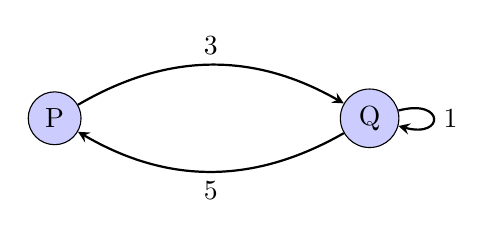
\begin{tikzpicture}[node distance=1.5cm, auto, >=stealth]
        \node[circle, draw, fill=blue!20] (A) at (0, 0) {P};
        \node[circle, draw, fill=blue!20] (C) at (4, 0) {Q};
        \draw[->, thick] (A) to[bend left] node[midway, above] {3} (C);
        \draw[->, thick] (C) to[bend left] node[midway, below] {5} (A);
        \draw[->, thick] (C) to[loop right] node[midway, right] {1} (C);
    \end{tikzpicture}
    \caption{Contoh graf berarah dan berbobot.}
    \label{contohgraf}
\end{figure}

\subsection{Matriks Adjacency dan Matriks Max-Plus}

Dalam graf berarah berbobot, matriks adjacency digunakan untuk merepresentasikan hubungan antar simpul. Setiap entri \( a_{ij} \) dalam matriks ini mewakili bobot pada sisi dari simpul \( i \) ke simpul \( j \), dan jika tidak ada sisi, maka bobotnya adalah elemen netral dalam aljabar max-plus, yaitu \( -\infty \) \cite{baccelli}.

Pada \ref{contohgraf}, matriks adjacency dari graf tersebut adalah:
\[
\begin{pmatrix}
    -\infty & 3 \\
    5 & 1
\end{pmatrix}
\]

\section{Nilai Eigen dan Vektor Eigen pada Aljabar Max-Plus}

Nilai eigen dan vektor eigen dalam aljabar max-plus merupakan konsep penting untuk menganalisis sistem linier dalam konteks aljabar ini. Definisi nilai eigen dan vektor eigen untuk suatu matriks \( A \in R_{\max}^{n \times n} \) diberikan sebagai berikut \cite{andro2020}:

\begin{definisi}
Diberikan \( A \in \Real_{\max}^{n \times n} \). Jika terdapat \( \lambda \in \Real_{\max} \) dan \( v \in R_{\max}^n \) dengan \( v \neq \epsilon \) sedemikian sehingga:
\[
A \otimes v = \lambda \otimes v,
\]
maka \( \lambda \) disebut nilai eigen matriks \( A \), dan \( v \) disebut vektor eigen yang bersesuaian dengan \( \lambda \).
\end{definisi}

\section{Sistem Persamaan Linear Max-Plus}

Sistem persamaan linear max-plus adalah model matematika untuk sistem peristiwa diskrit yang dapat dianalisis menggunakan operasi max-plus. Pendekatan ini memanfaatkan operasi maksimum (\(\oplus\)) dan penjumlahan biasa (\(\otimes\)) untuk menggantikan operasi penjumlahan dan perkalian pada aljabar klasik \cite{baccelli, heidergott}.

\begin{definisi}[Sistem Persamaan Linear Max-Plus]
Sistem persamaan linear max-plus adalah sistem yang dapat direpresentasikan dalam bentuk:
\[
x(k) = \bigoplus_{m=0}^M A_m \otimes x(k-m) \oplus B \otimes u(k)
\]
di mana \(x(k) \in \Real^{n \times 1}\) adalah vektor keadaan, \(u(k) \in \Real^{r \times 1}\) adalah vektor masukan, \(A_m \in \Real^{n \times n}\) adalah matriks keadaan, dan \(B \in \Real^{n \times r}\) adalah matriks input \cite{baccelli}.
\end{definisi}

\begin{definisi}[Matriks Kleene]
Untuk setiap matriks \(A \in \Real^{n \times n}\), matriks Kleene \(A^*\) didefinisikan sebagai:
\[
A^* = \bigoplus_{k=0}^\infty A^{\otimes k}
\]
dengan \(A^{\otimes k}\) menyatakan hasil perkalian matriks \(A\) sebanyak \(k\) kali dalam aljabar max-plus. Matriks ini digunakan untuk menyelesaikan sistem persamaan \((A \otimes x) \oplus b = x\) ketika graf \(G(A)\) memiliki bobot siklus rata-rata tidak positif \cite{subiono2015minmaxplus}.
\end{definisi}

\begin{teorema}[Penyelesaian Sistem Linear Max-Plus]
Jika \(A \in \Real^{n \times n}\) adalah matriks dengan bobot siklus rata-rata tidak positif, maka sistem:
\[
(A \otimes x) \oplus b = x
\]
memiliki solusi unik yang diberikan oleh:
\[
x = A^* \otimes b
\]
di mana \(A^*\) adalah matriks Kleene dari \(A\) \cite{baccelli}.
\end{teorema}

Sistem persamaan linear max-plus dapat direduksi menjadi bentuk rekursif sederhana:
\[
x(k+1) = A \otimes x(k)
\]
dengan \(A\) sebagai matriks transisi. Bentuk ini mempermudah analisis sistem seperti perhitungan nilai eigen dan vektor eigen yang menentukan sinkronisasi \cite{andro2020}.

\begin{teorema}[Nilai Eigen dan Vektor Eigen]
Untuk sebuah matriks \(A \in \Real^{n \times n}\), nilai eigen (\(\lambda\)) dan vektor eigen (\(v\)) memenuhi hubungan:
\[
A \otimes v = \lambda \otimes v
\]
di mana \(\lambda\) merepresentasikan periode sinkronisasi dan \(v\) menunjukkan pola stabil keadaan sistem \cite{baccelli}.
\end{teorema}

\section{Algoritma Power}
Menurut \citeauthor{andro2020}, setiap matriks \( A \) dalam aljabar max-plus memiliki setidaknya satu nilai eigen. Penentuan nilai eigen dan vektor eigen dapat dilakukan menggunakan algoritma \textit{Power}, yang dirumuskan dalam bentuk rekursi:
\[
x(k+1) = A \otimes x(k), \quad k = 0, 1, 2, \dots
\]

Algoritma ini terdiri dari langkah-langkah berikut:
\begin{enumerate}
     \item Berikan nilai awal \( x(0) \neq (\varepsilon, \varepsilon, \dots, \varepsilon)^T \).
        \item Iterasikan persamaan rekursif hingga terjadi perilaku periodik \( x(p) = c \otimes x(q) \), dengan \( p > q \geq 0 \).
        \item Hitung nilai eigen \( \lambda = c^{1/(p-q)} \).
        \item Tentukan vektor eigen menggunakan:
        \[
        v = \bigoplus_{i=1}^{p-q} \left( \lambda^{p-q-i} \otimes x(q+i-1) \right).
        \]
\end{enumerate}

Sistem persamaan linear max-plus memungkinkan analisis sistem diskrit dengan alat aljabar yang unik. Dengan pemanfaatan matriks Kleene, nilai eigen, dan algoritma iteratif, sistem ini sangat aplikatif dalam transportasi publik, produksi, dan jaringan telekomunikasi \cite{andro2020, subiono2015minmaxplus}.

\pagebreak
\chapter{METODOLOGI}
Pada bab ini akan dijelaskan secara umum mengenai urutan pelaksanaan Tugas Akhir dengan langkah-langkah yang dilakukan ditunjukkan pada diagram alir \ref{diagramalir}.
\begin{figure}[H]
	\centering
	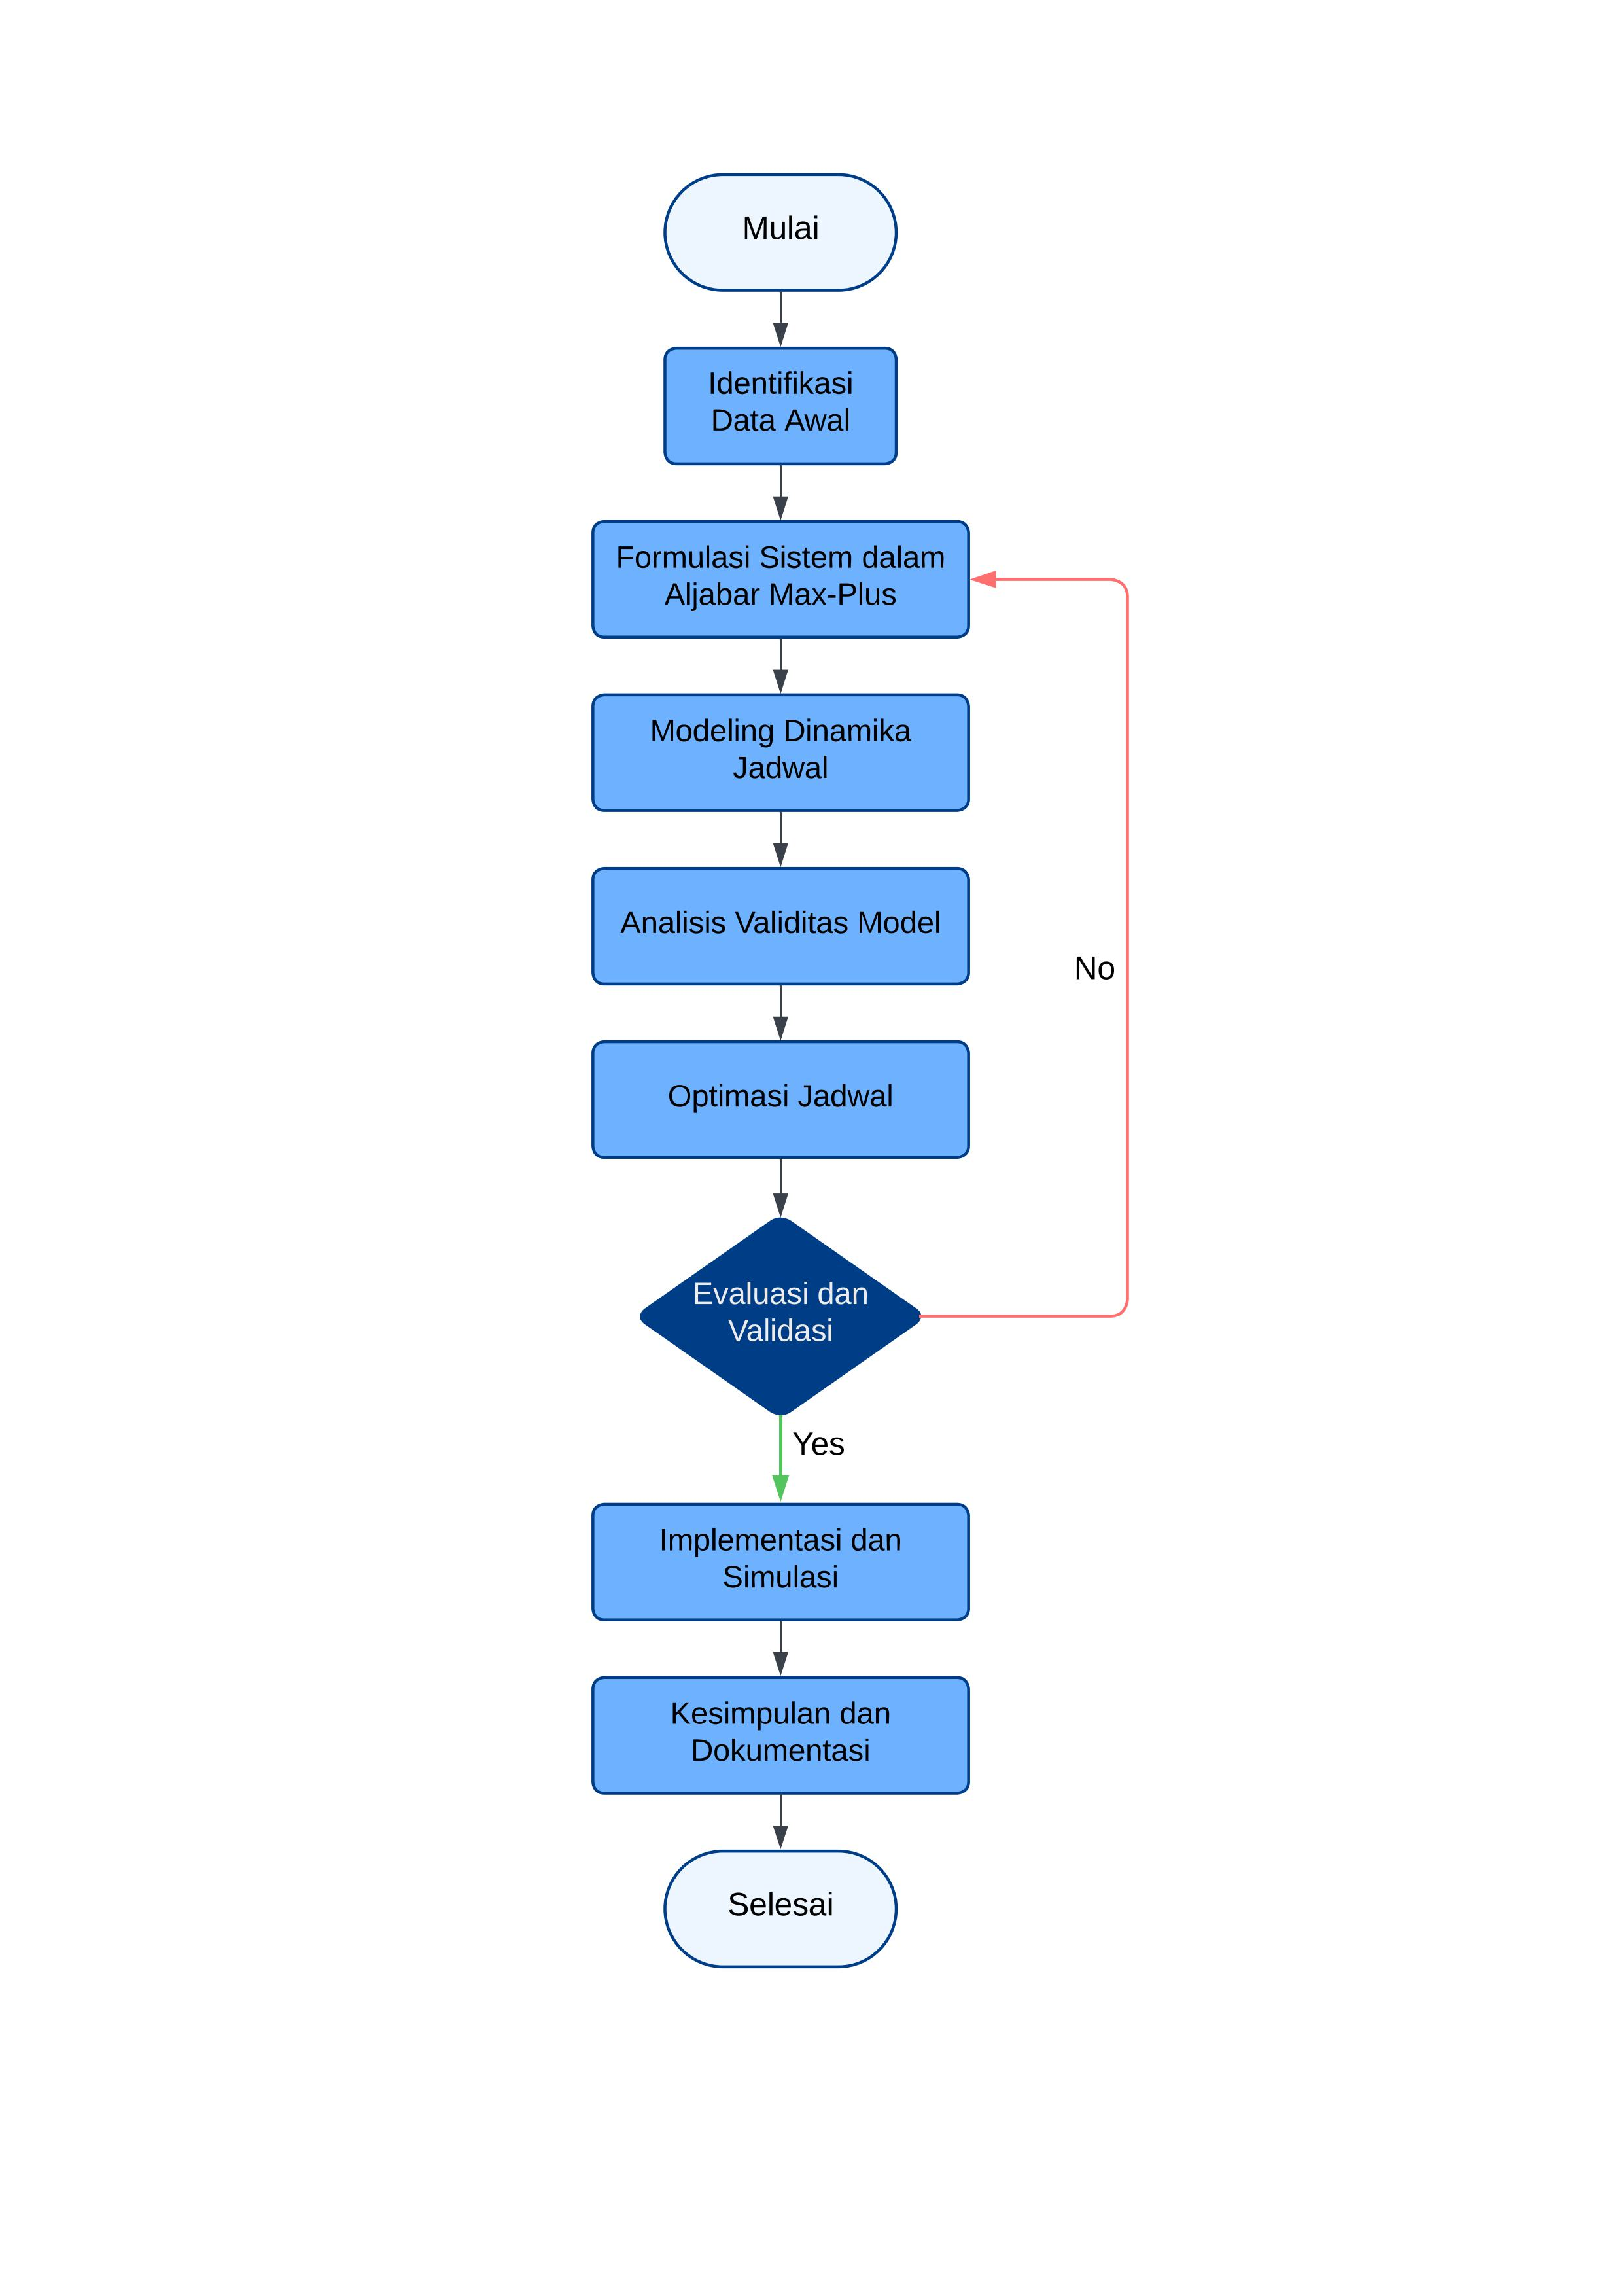
\includegraphics[trim={0 2cm 0 2cm},clip,scale=0.7]{foto/Diagram alir max plus.jpg}
	\caption{Diagram Alir Metodologi.}
	\label{diagramalir}
\end{figure}

\section{Identifikasi Data Awal}
Langkah pertama dalam penelitian ini adalah mengidentifikasi data awal yang relevan untuk membangun model. Data yang dikumpulkan meliputi parameter sistem yang akan digunakan dalam formulasi model serta pola waktu yang sesuai.

\section{Formulasi Sistem dalam Aljabar Max-Plus}
Setelah data awal diidentifikasi, sistem diformulasikan dalam kerangka aljabar Max-Plus. Langkah ini mencakup representasi elemen waktu dan operasi dalam bentuk matriks Max-Plus, yang mempermudah analisis dan optimasi jadwal.

\section{Modeling Dinamika Jadwal}
Berdasarkan formulasi Max-Plus, dinamika jadwal dimodelkan. Hal ini mencakup analisis perilaku sistem dalam berbagai kondisi input dan output, serta potensi pengaruh parameter waktu pada kinerja sistem.

\section{Analisis Validitas Model}
Langkah ini bertujuan untuk mengevaluasi validitas model yang telah dibangun. Apabila model tidak valid atau tidak sesuai dengan data dan sistem nyata, maka dilakukan perbaikan dan iterasi kembali ke tahap formulasi.

\section{Optimasi Jadwal}
Tahap berikutnya adalah melakukan optimasi terhadap jadwal berdasarkan model yang telah tervalidasi. Optimasi ini bertujuan untuk mencari solusi terbaik dalam penjadwalan yang sesuai dengan kriteria yang ditentukan.

\section{Evaluasi dan Validasi}
Hasil optimasi dievaluasi dan divalidasi untuk memastikan bahwa solusi yang diperoleh sesuai dengan tujuan penelitian. Jika evaluasi menunjukkan ketidaksesuaian, maka dilakukan revisi pada langkah sebelumnya.

\section{Implementasi dan Simulasi}
Setelah validasi berhasil, model diterapkan dan diuji melalui simulasi. Hasil simulasi akan memberikan gambaran tentang performa jadwal yang dioptimalkan dalam kondisi nyata.

\section{Kesimpulan dan Dokumentasi}
Langkah terakhir adalah merangkum hasil penelitian dalam bentuk kesimpulan dan mendokumentasikan seluruh proses dalam laporan tugas akhir.

\section{Jadwal Kegiatan}
Berikut ini disajikan tabel jadwal kegiatan yang akan dilakukan selama 3 bulan dan berkoresponden dengan metodologi.\vspace{0.5cm}

% Membuat tabel
\begin{table}[H]
\caption{Jadwal Kegiatan}
\centering
\begin{tabular}{|C{0.6cm}|L{5.7cm}|C{0.25cm}|C{0.25cm}|C{0.25cm}|C{0.25cm}|C{0.25cm}|C{0.25cm}|C{0.25cm}|C{0.25cm}|C{0.25cm}|C{0.25cm}|C{0.25cm}|C{0.25cm}|}
\hline
&&\multicolumn{12}{c|}{\textbf{BULAN}}\\\cline{3-14}
\multicolumn{1}{|c|}{\textbf{NO}}&\multicolumn{1}{c|}{\textbf{NAMA KEGIATAN}}&\multicolumn{4}{c|}{1}&\multicolumn{4}{c|}{2}&\multicolumn{4}{c|}{3}\\\cline{3-14}
&&1&2&3&4&1&2&3&4&1&2&3&4\\\cline{1-14}

1&Identifikasi Data Awal&\cellcolor{black!}&\cellcolor{black!}&&&&&&&&&&\\\hline
2&Formulasi Sistem dalam Aljabar Max-Plus&&&\cellcolor{black!}&\cellcolor{black!}&\cellcolor{black!}&&&&&&&\\\hline
3&Modeling Dinamika Jadwal&&&&&\cellcolor{black!}&\cellcolor{black!}&\cellcolor{black!}&&&&&\\\hline
4&Analisis Validitas Model&&&&&&&&\cellcolor{black!}&\cellcolor{black!}&\cellcolor{black!}&&\\\hline
5&Optimasi Jadwal&&&&&&&&\cellcolor{black!}&\cellcolor{black!}&\cellcolor{black!}&&\\\hline
6&Implementasi dan Simulasi&&&&&&&&&\cellcolor{black!}&\cellcolor{black!}&\cellcolor{black!}&\\\hline
7&Kesimpulan dan Dokumentasi&&&&&&&&&\cellcolor{black!}&\cellcolor{black!}&\cellcolor{black!}&\cellcolor{black!}\\\hline

\end{tabular}
\label{TabelJadwalKegiatan}
\end{table}
%%%%%%%%%%%%%%%%%%%%%%%%  Bab III  %%%%%%%%%%%%%%%5%%%%%%%%%%


%%%%%%%%%%%%%%%%%%%%%%%%  Dapus  %%%%%%%%%%%%%%%5%%%%%%%%%%

\pagebreak
\DaftarPustaka
%%%%%%%%%%%%%%%%%%%%%%%%  Dapus  %%%%%%%%%%%%%%%5%%%%%%%%%%
	
\end{document}